\documentclass[__main__.tex]{subfiles}

\begin{document}

\section{Вид явной разностной схемы для численного решения двумерного параболического уравнения (одна одномерная прогонка) в частных производных}

Рассмотрим задачу Коши:\\
\begin{gather}
\label{49.1}
\begin{cases}
\frac{\partial u}{\partial t} - \frac{\partial ^2 u}{\partial x^2} - \frac{\partial ^2 u}{\partial y^2} = f (x,y,t), & (x,y,t) \in (a,b) \times (c,d) \times (0,T];\\
u(x,y,0) = \mu (x,y), & (x,y) \in [a;b] \times [c;d];\\
u(a,y,t) = \alpha_a (y,t); \ u(b,y,t) = \alpha_b (y,t); & (y,t) \in [c;d] \times [0;T];\\
u(x,c,t) = \beta_c (x,t); \ u(x,d,t) = \beta_d (x,t); & (x,t) \in [a;b] \times [0;T]
\end{cases}
\end{gather}
Для исследования устойчивости конечно-разностных схем, использующихся для численного решения задачи \ref{49.1}, вместо этой задачи \ref{49.1} рассматривается однородная задача (без граничных условий) на числовой плоскости $R_2$:\\
\begin{gather}
\label{49.2}
\begin{cases}
\frac{\partial u}{\partial t} - \frac{\partial ^2 u}{\partial x^2} - \frac{\partial ^2 u}{\partial y^2} = 0, & (x,y,t) \in R_2 \times (0;T];\\
u(x,y,0) = \mu(x,y), & (x,y) \in R_2.
\end{cases}
\end{gather}
На плоскости $R_2$ задана сетка:\\
$$
C_1 = A \times B = <(x_i, y_j) = (h_x i, h_y j): (i,j) \in Z^2>
$$
На отрезке $[0;T]$ задана сетка:\\
$$
C_2 = <t^n = n \tau; n \in \overline{0,N}>
$$
Следовательно, будет использоваться сетка:\\
$$
C = C_1 \times C_2 = <(x_i, y_j, t^n) = (h_x i, h_y j, \tau n): (i,j) \in Z, n = \overline{0,N}>
$$
Для задачи \ref{49.2} будут использованы $C$-сеточные функции, которые в узлах сетки $C$ имеют вид:\\
\begin{gather}
\begin{cases}
u(x_i,y_j,t^n) = u_{ij}^n , & i,j \in Z \ \ \text{и} \ \ n = \overline{0,N};\\
\mu (x_i,y_j) = \mu_{ij} & \text{для} \ \ i,j \in Z
\end{cases}
\end{gather}
В этих обозначениях конечно-разностная схема (сеточный аналог) задачи \ref{49.2} примет вид, если использовать явную схему с шаблоном показанным на рисунке:\\
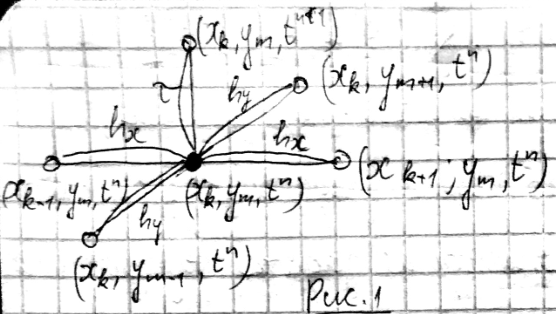
\includegraphics[width = 0.8\linewidth]{img_491}\\
\begin{gather}
\label{49.3}
\begin{cases}
\frac{u_{k,m}^{n+1} - u_{k,m}^{n}}{\tau} - \frac{u_{k-1,m}^{n} - 2u_{k,m}^{n} + u_{k+1,m}^{n}}{h_x^2} - \frac{u_{k,m-1}^{n} - 2u_{k,m}^{n} + u_{k,m+1}^{n}}{h_y^2} = 0, & k,m \in Z \ \ \text{и} \ \ n \in \overline{0,N-1};\\
u_{k,m} = \mu_{k,m}, & k,m \in Z
\end{cases}
\end{gather}
Вид схемы \ref{49.3} говорит о использовании для построения этой схемы двумерного оператора сеточной структуры с собственными функциями на сетке $C_1$, которые в узле $(x_k,y_m) = (kh_x,mh_y) \in C_1$ имеют вид: $e^{i(k\alpha + m\beta)}$, собственное значение $\lambda(\alpha,\beta)$.\\
\end{document}
